%%%%%%%%%%%%%%%%%%%%%%%%%%%%%%%%%%%%%%%%%
% Beamer Presentation
% LaTeX Template
% Version 1.0 (10/11/12)
%
% This template has been downloaded from:
% http://www.LaTeXTemplates.com
%
% License:
% CC BY-NC-SA 3.0 (http://creativecommons.org/licenses/by-nc-sa/3.0/)
%
%%%%%%%%%%%%%%%%%%%%%%%%%%%%%%%%%%%%%%%%%

%----------------------------------------------------------------------------------------
%	PACKAGES AND THEMES
%----------------------------------------------------------------------------------------

\documentclass{beamer}

\mode<presentation> {

% The Beamer class comes with a number of default slide themes
% which change the colors and layouts of slides. Below this is a list
% of all the themes, uncomment each in turn to see what they look like.

%\usetheme{default}
%\usetheme{AnnArbor}
%\usetheme{Antibes}
%\usetheme{Bergen}
%\usetheme{Berkeley}
%\usetheme{Berlin}
%\usetheme{Boadilla}
%\usetheme{CambridgeUS}
%\usetheme{Copenhagen}
%\usetheme{Darmstadt}
%\usetheme{Dresden}
%\usetheme{Frankfurt}
%\usetheme{Goettingen}
%\usetheme{Hannover}
%\usetheme{Ilmenau}
%\usetheme{JuanLesPins}
%\usetheme{Luebeck}
\usetheme{Madrid}
%\usetheme{Malmoe}
%\usetheme{Marburg}
%\usetheme{Montpellier}
%\usetheme{PaloAlto}
%\usetheme{Pittsburgh}
%\usetheme{Rochester}
%\usetheme{Singapore}
%\usetheme{Szeged}
%\usetheme{Warsaw}

% As well as themes, the Beamer class has a number of color themes
% for any slide theme. Uncomment each of these in turn to see how it
% changes the colors of your current slide theme.

%\usecolortheme{albatross}
%\usecolortheme{beaver}
%\usecolortheme{beetle}
%\usecolortheme{crane}
%\usecolortheme{dolphin}
%\usecolortheme{dove}
%\usecolortheme{fly}
%\usecolortheme{lily}
%\usecolortheme{orchid}
%\usecolortheme{rose}
%\usecolortheme{seagull}
%\usecolortheme{seahorse}
%\usecolortheme{whale}
%\usecolortheme{wolverine}
\setbeamertemplate{footline}[page number]
\setbeamertemplate{navigation symbols}{}
% To remove the footer line in all slides uncomment this line
%\setbeamertemplate{footline}[page number] % To replace the footer line in all slides with a simple slide count uncomment this line
%\setbeamertemplate{navigation symbols}{} % To remove the navigation symbols from the bottom of all slides uncomment this line
}

\usepackage{graphicx} % Allows including images
\usepackage{booktabs} % Allows the use of \toprule, \midrule and \bottomrule in tables

\usepackage{caption}
\usepackage{hyperref}
\usepackage{braket}

%----------------------------------------------------------------------------------------
%	TITLE PAGE
%----------------------------------------------------------------------------------------

\title{Shooting method for solving boundary value problems} % The short title appears at the bottom of every slide, the full title is only on the title page

\author{Shubham Raghuvanshi \\Harish Chandra Research Institute } % Your name


\date{\today} % Date, can be changed to a custom date

\begin{document}


\begin{frame}
\titlepage % Print the title page as the first slide
\end{frame}
\begin{frame}
	\frametitle{Solution of initial value problems}

	\begin{itemize}
		
		\item An m'th order ordinary differential equation of the form 
		
		\begin{equation}
		\frac{d^m y(t)}{d t^m} = f \left(t, y(t), \frac{d y(t)}{d t}, \frac{d^2 y(t)}{d t^2},...., \frac{d^{m-1} y(t)}{d t^{m-1}}      \right)
		\end{equation}
			
		can be converted to a system of 'm' coupled first order differential equations 

		\begin{equation}
		\frac{d y^{(n-1)}(t)}{dt} = y^{(n)}(t)  \text{     ,    } m \ge n \ge 1 		
		\end{equation}

by defining 'm+1' new variables $y^{(n)}(t)$,   $ 0 \le n \le m $ such that  
		
	\begin{equation}
	y^{(0)}(t) = y(t)
	\end{equation}
	\begin{equation}
	y^{(m)}(t) = f(t, y^{(0)}, y^{(1)}, y^{(2)},...., y^{(m-1)}   )
	\end{equation}
	
Which can be uniquely solved given 'm' initial conditions of the form 

\begin{equation}
     y^{(n)}(t_0) = a_n  \text{     ,    }  0 \le n \le m-1
\end{equation}

	\end{itemize}	
\end{frame}

\begin{frame}
	\frametitle{Methods of numerically solving IVP}
	
	Following are some of the well known methods for numerically solving IVP of the form
	
	\begin{equation}
	 \frac{d y}{dx} = f(x,y)
	\end{equation} 
	
	\begin{itemize}
		\item Euler's explicit and implicit method (Taylor series method of order 1) 
		\begin{eqnarray}
			y_{n+1} = y_{n} + \Delta x f(x_{n}, y_{n}) + O(\Delta x^2)\\
			y_{n+1} = y_{n} + \Delta x f(x_{n+1}, y_{n+1}) + O(\Delta x^2)\\
			y_{n+1} = y_{n} + \frac{\Delta x}{2} \left(  f(x_{n+1}, y_{n+1}) + f(x_{n}, y_{n})\right) + O(\Delta x^3)
		\end{eqnarray}
		\item Higher-order Taylor series methods
		\item $N^{th}$ order Runge-Kutta (RKN) methods.
		\begin{eqnarray}
		y_{n+1} = y_n +  \sum_{i=1}^{N}  w_i k_i\text{,      }  k_i  = h_n f \left( x_n + \alpha_i h_n, y_n + \sum_{j=1}^{i-1} \beta_{ij}k_j  \right)   
		\end{eqnarray}
		\item Predictor corrector methods
	\end{itemize}	
\end{frame}

\begin{frame}

\begin{center}
	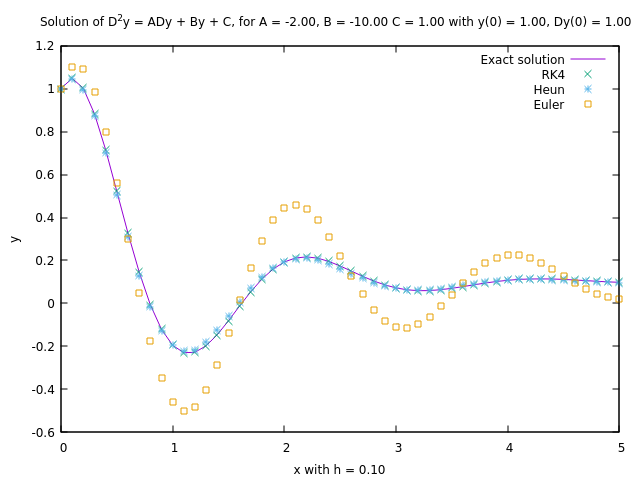
\includegraphics[width = 5.5cm , height = 5cm ]{2.png}
	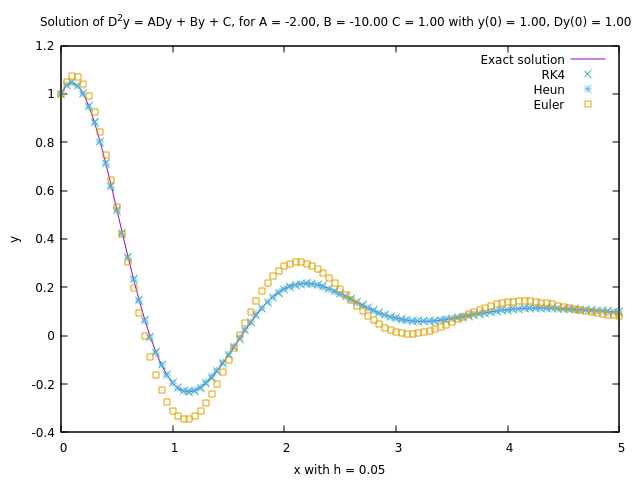
\includegraphics[width = 5.5cm , height = 5cm ]{1.png}\\
    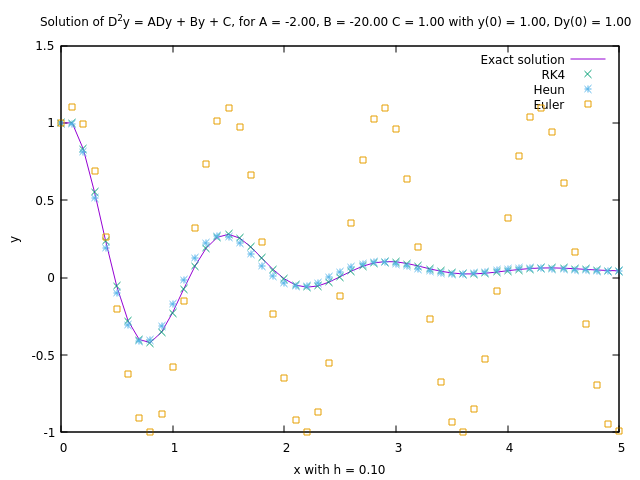
\includegraphics[width = 6cm , height = 4cm ]{3.png}
\end{center}
\end{frame}

\begin{frame}
	\frametitle{Shooting method for solving second order BVP}
	
	Consider a second order BVP 
	
	\begin{equation}
	y''(x) = f(x, y(x), y'(x) ) \text{     ,    } y(x_0) = y_0, y(x_1) = y_1
	\end{equation}
	
	Let $y(x;a)$ be the solution of the IVP 
	
	\begin{equation}
	y''(x) = f(x, y(x), y'(x) ) \text{     ,    } y(x_0) = y_0, y'(x_0) = a	
	\end{equation}
	
	Shooting method solves the BVP by finding the roots of the function 
	
	\begin{equation}
	F(a) = y(x_1, a) - y_1 
	\end{equation}
	
	The equation above can be solved numerically using any of numerical techniques such as Mid point method, Secant method etc. The shooting variable here is $y'(0)$, however it can be some other parameter as well e.g. $y(0)$ or Eigen values of TISE, 
	
\end{frame}

\begin{frame}
	\frametitle{Application: Particle in a box}
	
	The TISE for particle in a 1D infinite potential well can be written as a BVP 
	
	\begin{equation}
	\frac{d^2 \psi(x)}{d x^2} = - E \psi(x) \text{     ,    } \psi(0) = \psi(L) = 0   
	\end{equation}

     $ E_n  = n^2 \pi^2 $ are the eigenvalues. In order to solve for eigenfunctions one can fix $\psi(0), \psi'(0)$ and treat E as the shooting parameter.
	
	\begin{center}
		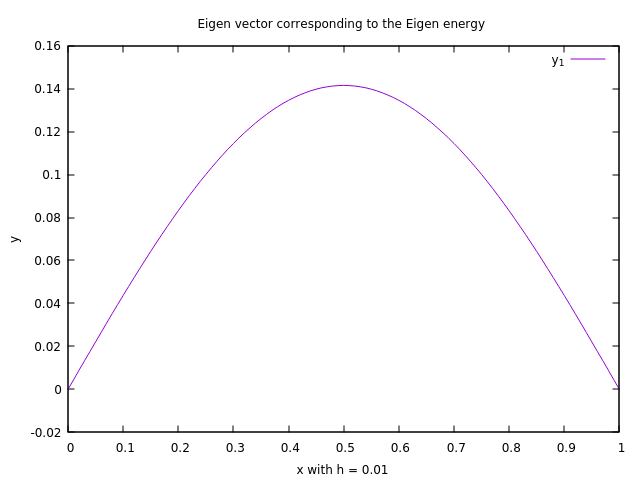
\includegraphics[width = 5.9cm , height = 4.8cm ]{5.png}
		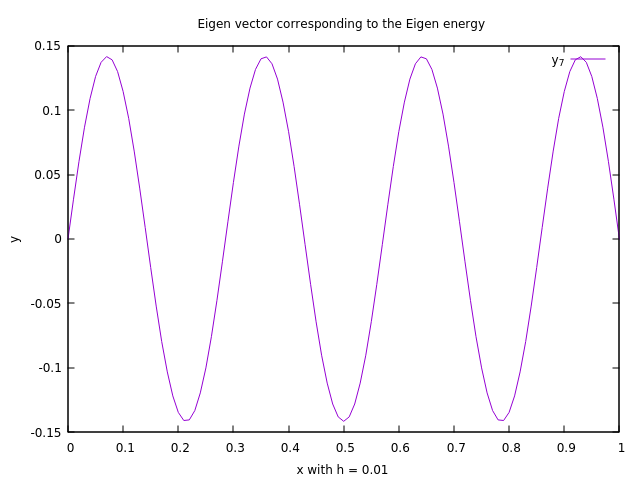
\includegraphics[width = 5.9cm , height = 4.8cm ]{8.png}
	\end{center}
		
\end{frame}


\begin{frame}
	\frametitle{Application: Quantum Harmonic Oscillator}
	
	The TISE  can be written as a BVP 
	
	\begin{equation}
	\frac{d^2 \psi(x)}{d x^2} = ( x^2 - E ) \psi(x) \text{     ,    } 
	\end{equation}
	
	Where the boundary conditions for odd and even solutions are $ \psi_{odd}(0)=0, \psi_{odd}(\infty) = 0$ and $ \psi'_{even}(0) = 0, \psi_{even}(\infty) = 0$.The eigenvalues are $ E_n  = 2n+1 $ .

	\begin{center}
	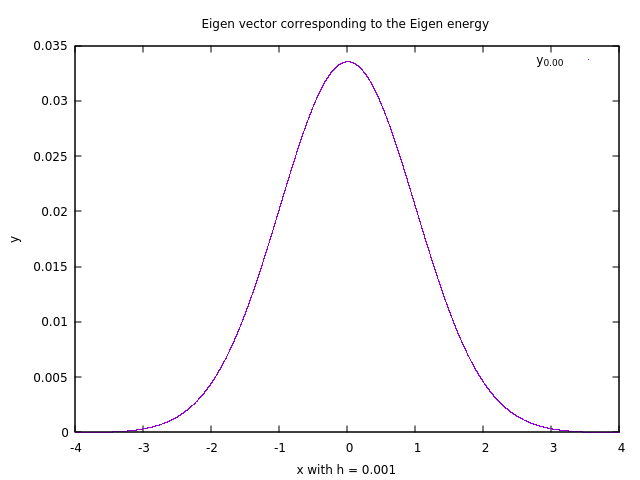
\includegraphics[width = 5.9cm , height = 4.8cm ]{7.png}
	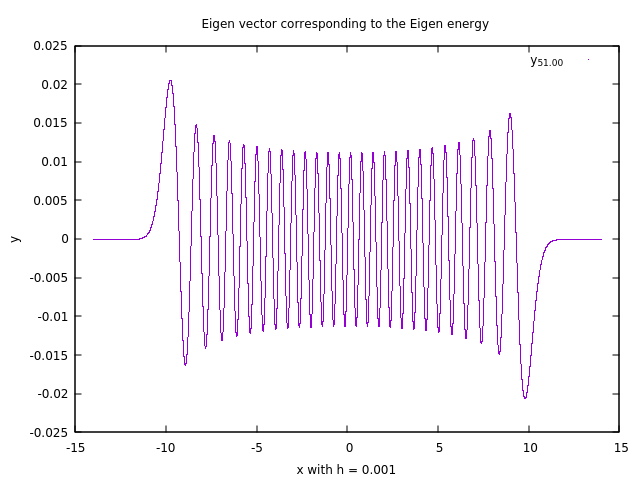
\includegraphics[width = 5.9cm , height = 4.8cm ]{9.png}
    \end{center}	
	
\end{frame}


\end{document} 






























